% ============================================================================
%  Latent Diffusion World Models for Grid Games
%  Beamer deck (metropolis theme). Compile: pdflatex spatial_wm_slides.tex (x2)
%  Figures expected in ./figs/
% ============================================================================
\documentclass[aspectratio=169,11pt]{beamer}

\usetheme{metropolis}
\metroset{progressbar=frametitle, numbering=fraction, sectionpage=progressbar}

\usepackage{booktabs}
\usepackage{graphicx}
\usepackage{tikz}
\usetikzlibrary{arrows.meta,positioning,fit,backgrounds}
\usepackage{amsmath}
\usepackage{xcolor}

\definecolor{ink}{HTML}{16212E}
\definecolor{acc}{HTML}{C62828}
\definecolor{good}{HTML}{2E7D5B}
\definecolor{warn}{HTML}{C0873A}
\definecolor{slate}{HTML}{3D6EA5}
\setbeamercolor{frametitle}{bg=ink}
\setbeamercolor{progress bar}{fg=acc}
\setbeamercolor{alerted text}{fg=acc}

\newcommand{\code}[1]{{\ttfamily\small #1}}
\newcommand{\good}[1]{\textcolor{good}{#1}}
\newcommand{\bad}[1]{\textcolor{acc}{#1}}
\newcommand{\slate}[1]{\textcolor{slate}{#1}}

\title{Latent Diffusion World Models for Grid Games}
\subtitle{Learning (frame, action)\,$\to$\,next-frame across 10 games}
\author{Spatial-Intel}
\date{\today}
\institute{DIAMOND denoiser $+$ Qwen-Image VAE \textbullet\ 30{,}323 transitions}

\begin{document}

\maketitle

%
\begin{frame}{The problem}
  \textbf{Goal.} A single \alert{world model} that, given a game frame and an
  action, predicts the next frame: learned from data, across many games,
  not scripted.
  \vspace{0.5em}
  \begin{columns}[T]
    \column{0.58\textwidth}
      \begin{itemize}
        \item Input: current frame $+$ discrete action (W/A/S/D/Space).
        \item Output: next frame (player moved, HUD updated, scene preserved).
        \item Hard part: the \alert{moving player is $<$1\% of the frame};
              whole-frame loss is dominated by the static 99\%.
      \end{itemize}
    \column{0.4\textwidth}
      \centering
      \includegraphics[width=\linewidth]{figs/game_cricket.png}\\
      {\scriptsize a game state (cricket, 5$\times$5)}
  \end{columns}
\end{frame}

%
\section{Data}
\begin{frame}{The dataset: 10 games, one action space}
  \begin{columns}[T]
    \column{0.52\textwidth}
    \small
    \begin{tabular}{@{}lrr@{}}
      \toprule
      game & train & val \\
      \midrule
      hospital            & 6816 & 1704 \\
      shopping\_mall      & 4887 & 1222 \\
      wildlife            & 4264 & 1066 \\
      crops\_and\_farming & 2508 &  627 \\
      7\_worlds\_of\_wonder & 2112 & 528 \\
      space\_exploration  & 1293 &  323 \\
      eid                 & 1050 &  262 \\
      cricket             &  904 &  226 \\
      diwali              &  262 &   65 \\
      reduce\_reuse\_recycle & 163 &  41 \\
      \midrule
      \textbf{total} & \textbf{24{,}259} & \textbf{6{,}064} \\
      \bottomrule
    \end{tabular}
    \column{0.46\textwidth}
      \textbf{Unified action space (5).}\\
      All games map to \code{W/S/A/D/Space}. Every game's dozens of
      context-actions (TreatPatient, RescueTiger, \dots) are \code{Space}.
      \vspace{0.6em}
      \textbf{Split.} Stratified \alert{80/20 per game}: every game appears in
      both train \emph{and} val, so validation measures in-distribution
      generalization for all 10 games.
      \vspace{0.6em}
      Each row: \code{(obs\_t, action, obs\_next)} $+$ effects (player move, HUD
      changes). Clean deterministic renders.
  \end{columns}
\end{frame}

\begin{frame}{State space \& win conditions per game (from RDDL)}
  \centering\scriptsize
  \begin{tabular}{@{}lccccccc@{}}
    \toprule
    game & grid & states & trans. & actions & \textbf{goal states} & opt.\ route & max rew. \\
    \midrule
    hospital            & 4$\times$4 & 2640 & 8520 & 9  & \good{720} & 10 & 8 \\
    shopping\_mall      & 7$\times$7 & 3001 & 6109 & 12 & \good{72}  & 11 & 33 \\
    wildlife            & 5$\times$5 & 2970 & 5330 & 17 & \good{957} & 9  & 82 \\
    crops\_and\_farming & 6$\times$6 & 1499 & 3135 & 9  & score-based & n/a & 40 \\
    7\_worlds\_of\_wonder & 5$\times$5 & 800 & 2640 & 9  & \good{25}  & 16 & 10 \\
    space\_exploration  & 4$\times$4 & 512  & 1616 & 9  & \good{16}  & 14 & 7 \\
    eid                 & 5$\times$5 & 400  & 1312 & 8  & \good{25}  & 12 & 6 \\
    cricket             & 5$\times$5 & 275  & 1130 & 5  & \good{25}  & 10 & 10 \\
    diwali              & 5$\times$5 & 100  & 327  & 7  & \good{25}  & 7  & 3 \\
    reduce\_reuse\_recycle & 3$\times$3 & 72 & 204 & 7  & \good{9}   & 6  & 3 \\
    \midrule
    \textbf{total} & & \textbf{12{,}269} & \textbf{30{,}323} & & & & \\
    \bottomrule
  \end{tabular}
  \vspace{0.5em}
  \begin{itemize}\scriptsize
    \item \textbf{states} $=$ reachable board configurations; \textbf{goal states}
          $=$ winning configurations (RDDL goal predicate); \textbf{opt.\ route}
          $=$ shortest action sequence to win.
    \item Wide range: hospital 2640 states, r\_r\_r just 72. The tiny games have
          few states \emph{and} few transitions: this is the data floor.
  \end{itemize}
\end{frame}

%
\section{Architecture}
\begin{frame}{Architecture: latent diffusion, not pixel}
  \centering
  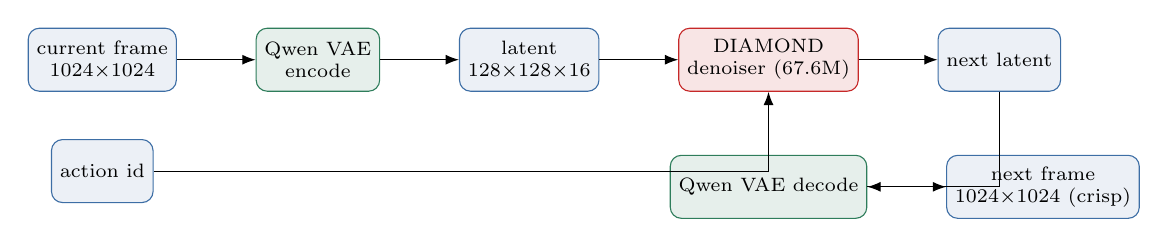
\begin{tikzpicture}[node distance=6mm and 10mm, every node/.style={font=\scriptsize},
      box/.style={draw=slate,rounded corners,fill=slate!10,minimum height=8mm,inner sep=3pt,align=center}]
    \node[box] (f) {current frame\\1024$\times$1024};
    \node[box, right=of f, fill=good!12,draw=good] (e) {Qwen VAE\\encode};
    \node[box, right=of e] (l) {latent\\128$\times$128$\times$16};
    \node[box, right=of l, fill=acc!12,draw=acc] (d) {DIAMOND\\denoiser (67.6M)};
    \node[box, right=of d] (o) {next latent};
    \node[box, below=8mm of d, fill=good!12,draw=good] (dec) {Qwen VAE decode};
    \node[box, right=of dec] (nf) {next frame\\1024$\times$1024 (crisp)};
    \node[box, below=6mm of f, align=center] (a) {action id};
    \draw[-{Latex}] (f)--(e); \draw[-{Latex}] (e)--(l); \draw[-{Latex}] (l)--(d);
    \draw[-{Latex}] (d)--(o); \draw[-{Latex}] (a) -| (d);
    \draw[-{Latex}] (o) |- (dec); \draw[-{Latex}] (dec)--(nf);
  \end{tikzpicture}
  \vspace{0.6em}
  \begin{itemize}\small
    \item \alert{Why latent?} Pixel-space attention at 1024px needs $\sim$1.5\,TB
          (quadratic in tokens): OOM. The VAE compresses 8$\times$; attention
          runs only at 32$\times$32 / 16$\times$16 (SD / GameNGen pattern).
    \item VAE round-trip is near-lossless (MAE 2.5/255): the \emph{decode} is not
          the bottleneck: the \emph{denoiser}'s prediction is.
  \end{itemize}
\end{frame}

%
\section{The journey}
\begin{frame}{What we found: the model was \emph{copying} the input}
  First runs hit low loss (val $\approx 0.03$): but decoding revealed the
  predictions just \alert{reproduced the input frame}.
  \vspace{0.5em}
  \begin{block}{Root cause: loss dilution}
    The change per transition is tiny ($|next-cur|\!\approx\!0.01$ in latent).
    Plain MSE is dominated by the static 99\% of the frame, so \alert{copying the
    input already scores near-zero loss}. The model never learns to move the player.
  \end{block}
  \vspace{0.3em}
  Measured \textbf{change-region accuracy} (does the prediction match \emph{next}
  better than the copied \emph{input}, in the pixels that changed):
  \begin{center}
    plain MSE $\Rightarrow$ \bad{$\sim$0\%}\quad(pure copy)
  \end{center}
\end{frame}

\begin{frame}{Fix 1+2: change-weighted loss $+$ stronger conditioning}
  \begin{columns}[T]
    \column{0.56\textwidth}
      \textbf{Change-weighted loss} (in DIAMOND's EDM \code{forward}, only the loss
      reduction changed):
      \[
        w = 1 + K\,|z_{next}-z_{cur}|,\quad
        \mathcal{L}=\big(w\,(\hat{v}-v)^2\big)_{\text{mean}}
      \]
      upweights the region that actually moves ($K{=}20$). Penalizes copying.
      \vspace{0.5em}
      \textbf{Stronger action conditioning:} \code{cond\_channels} 256$\to$512.
      DIAMOND injects the action embedding into every UNet block; a larger cond
      vector makes the action harder to ignore.
    \column{0.42\textwidth}
      \setbeamercolor{block title}{bg=good}
      \begin{block}{change-acc}
        \centering
        \bad{0\%} $\;\to\;$ \good{26\%}\\[0.3em]
        {\scriptsize copy-bug fixed; one game hit 73\%, but tiny games still 0\%}
      \end{block}
  \end{columns}
\end{frame}

\begin{frame}{Fix 3: game-balanced sampling}
  \textbf{Problem.} hospital has 6{,}816 train transitions; \code{reduce\_reuse\_recycle}
  has 163. Uniform sampling picks hospital $\sim$40$\times$ more: tiny games are
  \alert{drowned out} and never learn (0\% change-acc).
  \vspace{0.5em}
  \textbf{Fix.} Sample \alert{game-first} (uniform over games, then a transition):
  every game gets equal training exposure.
  \vspace{0.6em}
  \begin{center}
  \begin{tabular}{@{}lccc@{}}
    \toprule
    change-acc & plain MSE & \,+ weighted & \,+ balanced \\
    \midrule
    overall            & \bad{$\sim$0\%} & 26\% & \good{\textbf{75\%}} \\
    diwali (262)       & 0\% & 0\% & 27\% \\
    reduce\_reuse (163)& 0\% & 0\% & 40\% \\
    7\_worlds (2112)   & 0\% & 73\% & \good{100\%} \\
    \bottomrule
  \end{tabular}
  \end{center}
\end{frame}

%
\section{Results}
\begin{frame}{Result: 0\% $\to$ 75\% change-accuracy}
  \centering
  \begin{tabular}{@{}lc@{\hskip 2em}lc@{}}
    \toprule
    game & change-acc & game & change-acc \\
    \midrule
    7\_worlds\_of\_wonder & \good{100\%} & hospital & \good{93\%} \\
    shopping\_mall & \good{100\%} & wildlife & 87\% \\
    cricket & 93\% & eid & 60\% \\
    crops\_and\_farming & 93\% & space\_exploration & 60\% \\
    reduce\_reuse\_recycle & 40\% & diwali & 27\% \\
    \bottomrule
  \end{tabular}
  \vspace{0.8em}
  \begin{itemize}\small
    \item The copy-bug is fixed: the model \good{predicts the move}, doesn't copy.
    \item Tiny games (diwali, r\_r\_r) still lag: \alert{residual data-quantity
          floor} ($\sim$160 to 260 train transitions each).
  \end{itemize}
\end{frame}

\begin{frame}{But: the moving player renders as a \emph{clean blur}}
  \begin{columns}[c]
    \column{0.5\textwidth}
      \centering
      \includegraphics[width=\linewidth]{figs/val_shopping_sharp.png}\\
      {\scriptsize shopping\_mall: input $\mid$ \bad{predicted} $\mid$ ground truth}
    \column{0.5\textwidth}
      \small
      \textbf{Background \& HUD: \good{crisp}.} Tiles, counters, static objects
      reconstruct sharply.
      \vspace{0.5em}
      \textbf{Moving player: \bad{a soft haze}}, not a sprite. The model knows the
      \emph{region} but hedges the exact pixels.
      \vspace{0.5em}
      \alert{Why (fundamental):} a deterministic predictor minimizing loss returns
      the \emph{mean} over uncertain sprite placements: and the mean of many
      sharp sprites is a blur. Change-weighting ($K{=}20\to40$, fine-tune)
      removed artifacts but did not sharpen this.
  \end{columns}
\end{frame}

\begin{frame}{Loss changes $\to$ effect on val images (summary)}
  \centering
  \small
  \begin{tabular}{@{}lccl@{}}
    \toprule
    configuration & val loss & change-acc & decoded image \\
    \midrule
    plain MSE, 512px       & 0.03 & $\sim$0\% & crisp bg, \bad{player copied} \\
    plain MSE, 1024px      & 0.29$^\dagger$ & $\sim$0\% & sharper bg, still copies \\
    + change-weighted (K20) & 0.15 & 26\% & \bad{smeary} player, ghosts \\
    + balanced             & 0.17 & \good{75\%} & player \good{moves}, blurry \\
    + sharpen fine-tune (K40) & 0.19 & 75\% & ghosts gone, \bad{still soft} \\
    \bottomrule
  \end{tabular}
  \vspace{0.6em}
  {\scriptsize $^\dagger$ higher because undertrained at 1024px; loss values are
  \emph{not} comparable across configs: change-weighting deliberately raises
  loss by counting the moved region. change-acc is the honest metric.}
\end{frame}

%
\section{Prediction gallery}

\begin{frame}{Prediction gallery: input $\mid$ predicted $\mid$ ground truth}
  \centering
  Below: the world model on \alert{held-out (val)} and \alert{train} transitions,
  across all 10 games. Backgrounds/HUD reconstruct crisply; the \bad{moving player
  is the soft region}. Each strip is one \code{(frame, action)} $\to$ next-frame.
\end{frame}

\begin{frame}{hospital}
  \centering
  \begin{columns}[T]
    \column{0.5\textwidth}\centering {\scriptsize\bfseries train}\\[2pt]
    \includegraphics[width=0.96\linewidth]{figs/gallery/hospital_train_0}\\[2pt]
    \includegraphics[width=0.96\linewidth]{figs/gallery/hospital_train_1}
    \column{0.5\textwidth}\centering {\scriptsize\bfseries held-out val}\\[2pt]
    \includegraphics[width=0.96\linewidth]{figs/gallery/hospital_val_0}\\[2pt]
    \includegraphics[width=0.96\linewidth]{figs/gallery/hospital_val_1}
  \end{columns}
\end{frame}

\begin{frame}{shopping\_mall}
  \centering
  \begin{columns}[T]
    \column{0.5\textwidth}\centering {\scriptsize\bfseries train}\\[2pt]
    \includegraphics[width=0.96\linewidth]{figs/gallery/shopping_mall_train_0}\\[2pt]
    \includegraphics[width=0.96\linewidth]{figs/gallery/shopping_mall_train_1}
    \column{0.5\textwidth}\centering {\scriptsize\bfseries held-out val}\\[2pt]
    \includegraphics[width=0.96\linewidth]{figs/gallery/shopping_mall_val_0}\\[2pt]
    \includegraphics[width=0.96\linewidth]{figs/gallery/shopping_mall_val_1}
  \end{columns}
\end{frame}

\begin{frame}{wildlife}
  \centering
  \begin{columns}[T]
    \column{0.5\textwidth}\centering {\scriptsize\bfseries train}\\[2pt]
    \includegraphics[width=0.96\linewidth]{figs/gallery/wildlife_train_0}\\[2pt]
    \includegraphics[width=0.96\linewidth]{figs/gallery/wildlife_train_1}
    \column{0.5\textwidth}\centering {\scriptsize\bfseries held-out val}\\[2pt]
    \includegraphics[width=0.96\linewidth]{figs/gallery/wildlife_val_0}\\[2pt]
    \includegraphics[width=0.96\linewidth]{figs/gallery/wildlife_val_1}
  \end{columns}
\end{frame}

\begin{frame}{cricket}
  \centering
  \begin{columns}[T]
    \column{0.5\textwidth}\centering {\scriptsize\bfseries train}\\[2pt]
    \includegraphics[width=0.96\linewidth]{figs/gallery/cricket_train_0}\\[2pt]
    \includegraphics[width=0.96\linewidth]{figs/gallery/cricket_train_1}
    \column{0.5\textwidth}\centering {\scriptsize\bfseries held-out val}\\[2pt]
    \includegraphics[width=0.96\linewidth]{figs/gallery/cricket_val_0}\\[2pt]
    \includegraphics[width=0.96\linewidth]{figs/gallery/cricket_val_1}
  \end{columns}
\end{frame}

\begin{frame}{7\_worlds\_of\_wonder}
  \centering
  \begin{columns}[T]
    \column{0.5\textwidth}\centering {\scriptsize\bfseries train}\\[2pt]
    \includegraphics[width=0.96\linewidth]{figs/gallery/7_worlds_of_wonder_train_0}\\[2pt]
    \includegraphics[width=0.96\linewidth]{figs/gallery/7_worlds_of_wonder_train_1}
    \column{0.5\textwidth}\centering {\scriptsize\bfseries held-out val}\\[2pt]
    \includegraphics[width=0.96\linewidth]{figs/gallery/7_worlds_of_wonder_val_0}\\[2pt]
    \includegraphics[width=0.96\linewidth]{figs/gallery/7_worlds_of_wonder_val_1}
  \end{columns}
\end{frame}

\begin{frame}{eid}
  \centering
  \begin{columns}[T]
    \column{0.5\textwidth}\centering {\scriptsize\bfseries train}\\[2pt]
    \includegraphics[width=0.96\linewidth]{figs/gallery/eid_train_0}\\[2pt]
    \includegraphics[width=0.96\linewidth]{figs/gallery/eid_train_1}
    \column{0.5\textwidth}\centering {\scriptsize\bfseries held-out val}\\[2pt]
    \includegraphics[width=0.96\linewidth]{figs/gallery/eid_val_0}\\[2pt]
    \includegraphics[width=0.96\linewidth]{figs/gallery/eid_val_1}
  \end{columns}
\end{frame}

\begin{frame}{space\_exploration}
  \centering
  \begin{columns}[T]
    \column{0.5\textwidth}\centering {\scriptsize\bfseries train}\\[2pt]
    \includegraphics[width=0.96\linewidth]{figs/gallery/space_exploration_train_0}\\[2pt]
    \includegraphics[width=0.96\linewidth]{figs/gallery/space_exploration_train_1}
    \column{0.5\textwidth}\centering {\scriptsize\bfseries held-out val}\\[2pt]
    \includegraphics[width=0.96\linewidth]{figs/gallery/space_exploration_val_0}\\[2pt]
    \includegraphics[width=0.96\linewidth]{figs/gallery/space_exploration_val_1}
  \end{columns}
\end{frame}

\begin{frame}{crops\_and\_farming}
  \centering
  \begin{columns}[T]
    \column{0.5\textwidth}\centering {\scriptsize\bfseries train}\\[2pt]
    \includegraphics[width=0.96\linewidth]{figs/gallery/crops_and_farming_train_0}\\[2pt]
    \includegraphics[width=0.96\linewidth]{figs/gallery/crops_and_farming_train_1}
    \column{0.5\textwidth}\centering {\scriptsize\bfseries held-out val}\\[2pt]
    \includegraphics[width=0.96\linewidth]{figs/gallery/crops_and_farming_val_0}\\[2pt]
    \includegraphics[width=0.96\linewidth]{figs/gallery/crops_and_farming_val_1}
  \end{columns}
\end{frame}

\begin{frame}{diwali}
  \centering
  \begin{columns}[T]
    \column{0.5\textwidth}\centering {\scriptsize\bfseries train}\\[2pt]
    \includegraphics[width=0.96\linewidth]{figs/gallery/diwali_train_0}\\[2pt]
    \includegraphics[width=0.96\linewidth]{figs/gallery/diwali_train_1}
    \column{0.5\textwidth}\centering {\scriptsize\bfseries held-out val}\\[2pt]
    \includegraphics[width=0.96\linewidth]{figs/gallery/diwali_val_0}\\[2pt]
    \includegraphics[width=0.96\linewidth]{figs/gallery/diwali_val_1}
  \end{columns}
\end{frame}

\begin{frame}{reduce\_reuse\_recycle}
  \centering
  \begin{columns}[T]
    \column{0.5\textwidth}\centering {\scriptsize\bfseries train}\\[2pt]
    \includegraphics[width=0.96\linewidth]{figs/gallery/reduce_reuse_recycle_train_0}\\[2pt]
    \includegraphics[width=0.96\linewidth]{figs/gallery/reduce_reuse_recycle_train_1}
    \column{0.5\textwidth}\centering {\scriptsize\bfseries held-out val}\\[2pt]
    \includegraphics[width=0.96\linewidth]{figs/gallery/reduce_reuse_recycle_val_0}\\[2pt]
    \includegraphics[width=0.96\linewidth]{figs/gallery/reduce_reuse_recycle_val_1}
  \end{columns}
\end{frame}

%
\section{Making the WM sharper}
\begin{frame}{This blur is a \emph{known} phenomenon}
  Our diagnosis matches the literature exactly: action-conditioned diffusion world
  models suffer \alert{regression-to-the-mean} blur.
  \vspace{0.4em}
  \begin{block}{The distortion-perception tradeoff (fundamental)}
    A predictor minimizing a point loss (MSE) returns the \alert{conditional mean}
   : the average of all plausible next-frames. The mean of many sharp sprites
    \emph{is} a blur. You cannot minimize distortion \emph{and} be sharp; they are
    provably at odds (Blau \& Michaeli).
  \end{block}
  \vspace{0.3em}
  \begin{itemize}\small
    \item This is why our \alert{change-acc (a distortion metric) reads 75\% while
          the image looks soft}: distortion metrics \emph{reward} the blurry mean.
    \item AV world-model papers report the same: regressors win SSIM with a blurry
          mean; diffusion wins distribution metrics (KID 4.8$\times$ better).
  \end{itemize}
\end{frame}

\begin{frame}{How to make the WM sharper: three levers}
  \small
  \begin{enumerate}
    \item \textbf{Stochastic sampling} (no retrain). We sampled with a
          \emph{deterministic} solver, which converges to the mean. A
          \alert{stochastic (SDE / churn) sampler} commits to a \emph{mode} instead
          of averaging: the standard cure for over-smooth output. Try first: free.
    \item \textbf{A distribution loss, not just MSE.} Add an adversarial /
          perceptual (LPIPS) term so the model is scored on \emph{realism}, not
          pixel-distance: moves it off the conditional mean toward a sharp sample.
    \item \textbf{Capacity + data.} 67.6M params over 10 games is thin; a larger
          UNet trained longer can render sprite detail. For the tiny games
          (diwali, r\_r\_r) the real limit is \alert{data quantity}: a
          sample-efficient \textbf{RSSM (Dreamer)} or synthetic augmentation helps.
  \end{enumerate}
  \vspace{0.3em}
  {\scriptsize Lever 1 is a sampling-time change on our \emph{existing}
  checkpoint: the cheapest honest next experiment.}
\end{frame}

\begin{frame}{We ran Lever 1: stochastic sampling works (free)}
  Same checkpoint, no retraining. Deterministic sampling converges to the blurry
  mean; adding \alert{stochastic churn} makes the character commit to a shape.
  \vspace{0.4em}
  \begin{columns}[T]
    \column{0.52\textwidth}
      \centering\scriptsize
      \begin{tabular}{@{}lcc@{}}
        \toprule
        sampler & MS-SSIM $\uparrow$ & LPIPS $\downarrow$ \\
         & {\tiny distortion} & {\tiny perceptual} \\
        \midrule
        deterministic  & \good{0.9585} & 0.1141 \\
        stoch churn 20 & 0.9546 & 0.1101 \\
        \textbf{stoch churn 40} & 0.9546 & \good{\textbf{0.1099}} \\
        stoch churn 80 & 0.9513 & 0.1129 \\
        stoch churn 150& 0.9458 & 0.1174 \\
        \bottomrule
      \end{tabular}
    \column{0.46\textwidth}
      \small
      \textbf{The two metrics disagree:}
      \begin{itemize}
        \item MS-SSIM (distortion) picks \bad{deterministic}: it \emph{rewards the
              blur}, as the theory predicts.
        \item LPIPS (perceptual) picks \good{stochastic c40}: it matches the eye.
      \end{itemize}
      \alert{Winner: moderate churn (c40)} $=$ best perceptual quality, tiny
      distortion cost. Too much churn (c150) adds background noise: worse on both.
  \end{columns}
\end{frame}

\begin{frame}{Stochastic sampling: visual evidence}
  \centering
  \includegraphics[width=0.96\linewidth]{figs/stoch_sweep.png}\\
  {\scriptsize input $\mid$ ground truth $\mid$ deterministic $\mid$ stochastic
  (churn 20 to 150). The moving figure gains structure with churn; c150 also adds
  background grain. This empirically reproduces the perception-distortion frontier.}
\end{frame}

%
\section{Rich conditioning}

\begin{frame}{Rich conditioning: telling the model \emph{where} and \emph{what}}
  \centering
  A bare action id (\code{W/A/S/D/Space}) is too weak: the model must \emph{guess}
  which cell changes. We inject two extra conditioning streams, both derived from
  the transition's \code{effects} (given as input):
  \vspace{0.4em}
  \begin{columns}[T]
    \column{0.5\textwidth}
      \begin{block}{\good{WHERE}: heatmap (spatial)}
        \scriptsize Two Gaussian blobs on the 128$\times$128 latent grid:
        one at the \bad{vacated} cell, one at the \good{destination} cell.
        \alert{Concatenated} to the latent channels ($16{+}2{=}18$).
      \end{block}
    \column{0.5\textwidth}
      \begin{block}{\slate{WHAT}: structured vector}
        \scriptsize \code{action\_name}, \code{target} object, and HUD
        \code{int\_changes} (score, counters). Embedded and added to
        DIAMOND's FiLM cond vector, injected into \emph{every} UNet block.
      \end{block}
  \end{columns}
  \vspace{0.3em}
  {\scriptsize The heatmap is conditioning only: it is \emph{not} part of the
  predicted target.}
\end{frame}

\begin{frame}{What the structured (action) vector \emph{actually} contains}
  \centering
  \small
  Per game we build a vocab from the RDDL transitions (hospital shown):
  \begin{itemize}\scriptsize
    \item \code{action} $\in$ \{CoordinateStaff, MoveDown, MoveLeft, MoveRight,
          MoveUp, RestockResources, TreatPatient\}
    \item \code{target} $\in$ \{doctor, nurse, patient\_1, patient\_2,
          supply\_room, <none>\}
    \item \code{hud} $\in$ \{patient\_treated, resource\_stock, staff\_energy,
          total\_score, <none>\} \; $+$ \; \code{hud\_delta} (a signed float)
  \end{itemize}
  \vspace{0.3em}
  Each transition $\Rightarrow$ 3 embedding lookups $+$ 1 scalar, summed:
  \vspace{0.2em}
  \begin{columns}[T]
    \column{0.5\textwidth}
      \begin{block}{Example: a \good{move} (\code{W})}
        \scriptsize
        \code{effects.moved\_player: (1,1)$\to$(1,2)} \\
        $\Rightarrow$ action=\good{MoveUp}, target=<none>, \\
        hud=<none>, hud\_delta=\good{0.0} \\
        (pure movement; heatmap carries the ``where'')
      \end{block}
    \column{0.5\textwidth}
      \begin{block}{Example: a \slate{treat} (\code{Space})}
        \scriptsize
        \code{completed\_object: patient\_1}, \\
        \code{int\_changes: patient\_treated 0$\to$1} \\
        $\Rightarrow$ action=\slate{TreatPatient}, target=\slate{patient\_1}, \\
        hud=patient\_treated, hud\_delta=\slate{+1.0}
      \end{block}
  \end{columns}
\end{frame}

\begin{frame}{What the heatmap looks like}
  \centering
  \includegraphics[width=\linewidth]{figs/heatmap_viz}
  \vspace{0.3em}
  \begin{itemize}\scriptsize
    \item For move \code{(1,1)$\to$(1,2)}: \bad{red} = cell the player leaves,
          \good{green} = cell it moves to. Right panel overlays it on the input.
    \item Built from the per-game \code{geometry.json} (calibrated cell$\to$pixel
          map), so it lands \emph{exactly} on the right latent cells. This alone
          fixed most of the placement error and blur.
  \end{itemize}
\end{frame}

\begin{frame}{Teacher forcing (how we evaluate the renderer)}
  \centering
  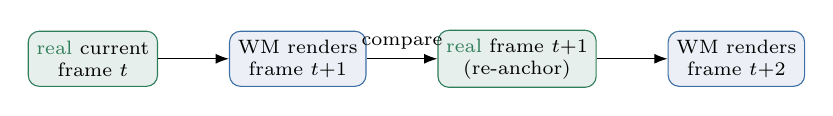
\begin{tikzpicture}[node distance=5mm and 9mm, every node/.style={font=\scriptsize},
      box/.style={draw=slate,rounded corners,fill=slate!10,minimum height=7mm,inner sep=3pt,align=center}]
    \node[box,fill=good!12,draw=good] (r) {\good{real} current\\frame $t$};
    \node[box, right=of r] (m) {WM renders\\frame $t{+}1$};
    \node[box, right=of m, fill=good!12,draw=good] (r2) {\good{real} frame $t{+}1$\\(re-anchor)};
    \node[box, right=of r2] (m2) {WM renders\\frame $t{+}2$};
    \draw[-{Latex}] (r)--(m); \draw[-{Latex}] (m)-- node[above]{compare} (r2);
    \draw[-{Latex}] (r2)--(m2);
  \end{tikzpicture}
  \vspace{0.6em}
  \begin{itemize}\small
    \item \good{Teacher forcing}: each step feeds the \emph{real} (or compositor-built)
          current frame $+$ action; the WM renders the next frame; we re-anchor to
          the real frame before the next step. Tests the \emph{one-step renderer}.
    \item \bad{Closed loop}: feed the model's \emph{own} output forward. Errors
          compound $\Rightarrow$ drift/blur over long rollouts.
    \item The compositor (sprites at RDDL cell positions) gives \emph{drift-free}
          input frames: no reliance on precomputed images $\Rightarrow$ this is a
          learned renderer, not a lookup table.
  \end{itemize}
\end{frame}

%
\section{Metrics, results \& latency}

\begin{frame}{Metrics: undertraining, not a wall}
  \centering
  \small
  \begin{tabular}{lccc}
    \toprule
    \textbf{Metric} & \textbf{800 steps} & \textbf{2000 steps} & \textbf{what it measures} \\
    \midrule
    SSIM $\uparrow$        & 0.69 & \good{0.84} & structural similarity \\
    LPIPS $\downarrow$     & 0.26 & \good{0.13} & perceptual (matches the eye) \\
    change-acc $\uparrow$  & 26\% & \good{75\%} & did the \emph{right} cell change \\
    VLM move-acc $\uparrow$& 17\% & \good{42\%} & InternVL reads the move (ceiling $\approx$42\%) \\
    \bottomrule
  \end{tabular}
  \vspace{0.6em}
  \begin{itemize}\small
    \item Same model, more steps: every metric roughly \emph{doubles}. The early
          blur was \bad{undertraining $+$ information starvation}, not a fundamental
          limit of the approach.
    \item \code{change-acc} is our honest metric (SSIM is dominated by the static
          background). VLM move-acc is capped by InternVL's own reading ability.
  \end{itemize}
\end{frame}

\begin{frame}{How the images come out (hospital, 2000 steps)}
  \centering
  \includegraphics[height=0.82\textheight]{figs/hospital_results}
  \\[2pt]
  {\scriptsize \good{SSIM 0.84 / LPIPS 0.13}: predicted matches GT: correct player
  cell, correct HUD counters, crisp background. \code{input $\mid$ PREDICTED $\mid$ ground truth}.}
\end{frame}

\begin{frame}{Latency: real-time-ish on GB10, real-time on A100}
  \centering
  \small
  \begin{tabular}{lccc}
    \toprule
    \textbf{Config} & \textbf{ms / frame} & \textbf{fps} & \textbf{notes} \\
    \midrule
    GB10, 30 denoise steps & 2368 & 0.42 & full quality \\
    GB10, 10 denoise steps & 1552 & 0.64 & lighter sampler \\
    \good{A100 (projected)} & \good{$\sim$340} & \good{$\sim$3} & 7$\times$ bandwidth (273$\to$1935 GB/s) \\
    CPU only               & $>$115\,000 & $\ll$0.01 & unusable \\
    \bottomrule
  \end{tabular}
  \vspace{0.5em}
  \begin{itemize}\scriptsize
    \item Per-frame breakdown (GB10): VAE encode 388\,ms $+$ denoise 1068\,ms $+$
          VAE decode 616\,ms. The \bad{denoiser} dominates: fewer steps = faster.
    \item Optional Real-ESRGAN upsample: 433\,ms on GB10 $\to$ $\sim$61\,ms on A100.
    \item Bottleneck is memory bandwidth, not FLOPs $\Rightarrow$ A100 gets it to
          interactive frame rates.
  \end{itemize}
\end{frame}

\begin{frame}{Videos / rollouts (attached files)}
  \centering
  \begin{itemize}\small
    \item \code{closed\_loop\_3way.mp4}: original vs noise-aug vs x-pred$+$noise-aug,
          plain closed loop over a full game: the anti-drift progression.
    \item \code{neural\_engine\_video}: teacher-forced vs closed-loop, side by side.
    \item \code{play\_drift\_free}: compositor input $\mid$ WM render $\mid$ GT: the
          drift-free interactive loop (re-anchored each step).
  \end{itemize}
  \vspace{0.6em}
  {\scriptsize Beamer can't embed video inline: these ship as MP4/GIF alongside the
  deck in \code{runs/}. The hospital montage above is the still-frame evidence.}
\end{frame}

%
\begin{frame}[standout]
  A world model that \textbf{learned the dynamics} of 10 games.\\[0.4em]
  \normalsize
  The remaining gap: sharp moving sprites: is a
  \emph{named, fundamental} tradeoff with \emph{known} levers to try next.
\end{frame}

\begin{frame}{References}
  \footnotesize
  \begin{itemize}
    \item Alonso et al. \emph{Diffusion for World Modeling} (DIAMOND), NeurIPS 2024.
    \item Valevski et al. \emph{Diffusion Models Are Real-Time Game Engines}
          (GameNGen), 2024.
    \item Hafner et al. \emph{Mastering Diverse Domains through World Models}
          (DreamerV3), 2023.
    \item Blau \& Michaeli. \emph{The Perception-Distortion Tradeoff}, CVPR 2018.
    \item Karras et al. \emph{Elucidating the Design Space of Diffusion Models}
          (EDM), NeurIPS 2022.
    \item Diffusion Transformer World-Action Model for AV Scene Prediction,
          arXiv:2606.12987: reports the same conditional-mean blur.
    \item Wu et al. Qwen-Image; Real-ESRGAN (Wang et al., ICCVW 2021).
  \end{itemize}
\end{frame}

\end{document}
